
% License:
% CC BY-NC-SA 3.0 (http://creativecommons.org/licenses/by-nc-sa/3.0/)
%
%%%%%%%%%%%%%%%%%%%%%%%%%%%%%%%%%%%%%%%%%

%----------------------------------------------------------------------------------------
%	PACKAGES AND OTHER DOCUMENT CONFIGURATIONS
%----------------------------------------------------------------------------------------
\newcommand{\virg}[1]{``#1''}
\documentclass[paper=a4, fontsize=11pt]{scrartcl} % A4 paper and 11pt font size
\usepackage{hyperref}
\usepackage{multirow}
\usepackage{fancyvrb}
\usepackage{geometry}
\usepackage{verbatim}
\geometry{left=2cm, right=2cm, top=2.5cm, bottom=2.5cm}
\usepackage{listings}
\usepackage{cancel}
\usepackage[T1]{fontenc} % Use 8-bit encoding that has 256 glyphs
\usepackage{fourier} % Use the Adobe Utopia font for the document - comment this line to return to the LaTeX default
\usepackage[italian]{babel} % English language/hyphenation
\usepackage{amsmath,amsfonts,amsthm} % Math packages
\usepackage{lipsum} % Used for inserting dummy 'Lorem ipsum' text into the template

\usepackage{caption}
\usepackage{subcaption}
\usepackage{graphicx}
\usepackage[font=small,labelfont=bf]{caption}
\usepackage{float}

\usepackage{blindtext} %for enumarations

\usepackage{algorithm}
\usepackage[noend]{algpseudocode}

\makeatletter
\def\BState{\State\hskip-\ALG@thistlm}
\makeatother


\usepackage[]{hyperref}  %link collor

%talbe layout to the right
%\usepackage[labelfont=bf]{caption}
%\captionsetup[table]{labelsep=space,justification=raggedright,singlelinecheck=off}
%\captionsetup[figure]{labelsep=quad}

\usepackage{sectsty} % Allows customizing section commands
\allsectionsfont{\centering \normalfont\scshape} % Make all sections centered, the default font and small caps

\usepackage{fancyhdr} % Custom headers and footers
\pagestyle{fancyplain} % Makes all pages in the document conform to the custom headers and footers
\fancyhead{} % No page header - if you want one, create it in the same way as the footers below
\fancyfoot[L]{} % Empty left footer
\fancyfoot[C]{} % Empty center footer
\fancyfoot[R]{\thepage} % Page numbering for right footer
\renewcommand{\headrulewidth}{0pt} % Remove header underlines
\renewcommand{\footrulewidth}{0pt} % Remove footer underlines
\setlength{\headheight}{13.6pt} % Customize the height of the header

\newcommand{\mbf}[1]{\mathbf{#1}}
\newcommand{\norm}[1]{\left\lVert#1\right\rVert}


\numberwithin{equation}{section} % Number equations within sections (i.e. 1.1, 1.2, 2.1, 2.2 instead of 1, 2, 3, 4)
\numberwithin{figure}{section} % Number figures within sections (i.e. 1.1, 1.2, 2.1, 2.2 instead of 1, 2, 3, 4)
\numberwithin{table}{section} % Number tables within sections (i.e. 1.1, 1.2, 2.1, 2.2 instead of 1, 2, 3, 4)

%\setlength\parindent{0pt} % Removes all indentation from paragraphs - comment this line for an assignment with lots of text


\setlength\parskip{4pt}

%----------------------------------------------------------------------------------------
%	TITLE SECTION
%----------------------------------------------------------------------------------------

\newcommand{\horrule}[1]{\rule{\linewidth}{#1}} % Create horizontal rule command with 1 argument of height

\title{	
\normalfont \normalsize 
\textsc{\huge University of Pisa} \\ [25pt] % Your university, school and/or department name(s)
\horrule{2pt} \\[0.5cm]
\huge Risoluzione di un problema di Constrained Convex Quadratic Programming con Primal-Dual Interior Point Method\\ % The assignment title
\horrule{0.5pt} \\[0.4cm] % Thin top horizontal rule
Computational Mathematics for Learning\\and Data Analysis project report\\
\horrule{2pt} \\[0.5cm] % Thick bottom horizontal rule
}

\author{Cornacchia Giuliano, Salinas Mario Leonardo\\Gruppo 21} % Your name

\date{} % Today's date or a custom date

\begin{document}
%\nocite{*}
\maketitle

\newpage
\tableofcontents
\newpage

%intro
\section{Introduzione}

Nel seguente report viene descritto ed analizzato il problema numero 3 \emph{noML} assegnato per il progetto finale di \emph{Computational Mathematics for Learning and Data Analysis} e descritta la soluzione da noi proposta, insieme alle varie scelte implementative.

%problem description
\section{Descrizione del problema}

Date le matrici $Q \in \mathbb{R}^{n \times n}$ ed $A \in \lbrace0, 1\rbrace^{k\times n}$, con $Q\succeq 0$, e i vettori $q\in\mathbb{R}^n$ e $b=[1]^k$, il problema di ottimizzazione quadratica convessa primale $P$ è definito come:

\begin{equation} \label{eq:primal_problem}
P := \begin{cases} {min }\;\; x^\intercal Qx+q^\intercal x \\ Ax=b \\x\geq 0\end{cases}
\end{equation}

dove i vincoli nella matrice $A$ formano $k$ simplessi disgiunti della forma:

\begin{equation} \label{eq:vincoli}
\sum_{i \in I^h} x_i = 1, h = 1, \dots, k
\end{equation}

con $I^h, h = 1, \dots, k$ insiemi di indici che formano una partizione di $\{1,\dots,n\}$. Quindi il generico elemento della matrice $A$ $a_{vi} = 1 \Longleftrightarrow i \in I^v$.

Data la funzione da minimizzare in \ref{eq:primal_problem} $f(x) = x^\intercal Qx +q^\intercal x$ e la sua \emph{funzione Lagrangiana} $L(x,\lambda_{eq}, \lambda_s)$, a $P$ si può associare il seguente \emph{Problema Duale di Wolfe} $D$:

\begin{equation} \label{eq:dual_problem}
D := \begin{cases}\mathrm{max} \;\; L(x,\lambda_{eq},\lambda_s)\\
\nabla _x L(x, \lambda_{eq}, \lambda_s) = 0 \\
\lambda_s \geq 0
\end{cases}
= 
\begin{cases} \mathrm{max}\;\;  x^\intercal Qx +q^\intercal x + \lambda^\intercal_{eq}(Ax - b) +\lambda^\intercal_s(-x)\\
2Qx + q + A^\intercal \lambda_{eq} -\lambda_s= 0 \\
\lambda_s \geq 0
\end{cases}
\end{equation}

Possiamo a questo punto scrivere il sistema KKT associato a $P$.

\begin{equation} \label{eq:kkt}
    \begin{cases}\nabla _x L(x, \lambda_{eq}, \lambda_s) = 0 \\
        Ax - b = 0\\
        x_i  \lambda_{s_i} = 0 \;\;\;\;\;\;\; i = 1, \dots, n \\
        (x,\lambda_s) \geq 0
    \end{cases}
\end{equation}

\begin{comment}
\rightarrow
\begin{bmatrix}
\nabla _x L(x, \lambda_{eq}, \lambda_s)\\Ax - b\\XSe
\end{bmatrix}
=
\begin{bmatrix}
0\\ 0 \\0
\end{bmatrix}
\rightarrow
\begin{bmatrix}
2Q & A^\intercal & -I\\
A & 0 & 0 \\
S & 0 & X
\end{bmatrix}
\;
\begin{bmatrix}
x \\ \lambda_{eq} \\ \lambda_s
\end{bmatrix}
=
\begin{bmatrix}
-q\\ b \\ 0
\end{bmatrix}
\end{comment}

Scegliamo dunque di risolvere il sistema \ref{eq:kkt} applicando il metodo Primal-Dual Interior Point (PDIP): riformuliamo le condizioni di ottimalità \ref{eq:kkt} 
definendo una funzione $F : \mathbb{R}^{2n+k} \rightarrow \mathbb{R}^{2n+k}$ \cite{Nocedal2006Numerical}:
\begin{subequations}
\begin{equation} \label{eq:F}
F(x, \lambda_{eq}, \lambda_s)=
\begin{bmatrix}
\nabla _x L(x, \lambda_{eq}, \lambda_s)\\Ax - b\\XSe
\end{bmatrix}
=0
\end{equation}
\begin{equation} \label{eq:nonneg}
\;\;\;\;\;\;\;\;\;\;\;\;\;\;\;\;\;\;\;\;\;\;\;\;\;\;\;\;\;\;\;\;\;\;\;\;\;\;\;\;\;\;\;\;\;\;\;\;\;\;\;\;\;\;\;\;\;\;\;\;\;\;(x,\lambda_s)\geq 0
\end{equation}
\end{subequations}
dove

\begin{equation} \label{eq:xs}
    X = diag(x_1, \dots, x_n) \;\;\;\;\;\;\;\;\;\;\;\; 
    S = diag(\lambda_{s_1}, \dots, \lambda_{s_n}) \;\;\;\;\;\;\;\;\;\;\;\; 
    e^\intercal = [1, \dots, 1] \in \mathbb{R}^n
\end{equation}

Il metodo PDIP, ad ogni iterazione $k$, genera triple $(x^k, \lambda_{eq}^k, \lambda_{s}^k)$ 
che soddisfano \emph{strettamente} la \ref{eq:nonneg}.\\
La procedura con la quale si ricercano le direzioni $(\Delta x, \Delta \lambda_{eq}, \Delta \lambda_s)$ 
prende origine dal metodo di Newton per equazioni non lineari \cite{Nocedal2006Numerical}: 
alla $k$-esima iterazione il metodo di Newton forma un modello lineare di $F$ 
attorno al punto corrente $(x^k, \lambda_{eq}^k, \lambda_{s}^k)$ e ottiene 
le direzioni di ricerca risolvendo il seguente sistema lineare:

\begin{equation} \label{eq:J}
J(x, \lambda_{eq}, \lambda_s) \begin{bmatrix}
\Delta x \\ \Delta \lambda_{eq}\\ \Delta \lambda_s
\end{bmatrix} = -F(x, \lambda_{eq}, \lambda_{s})
\end{equation}

dove $J$ è la Jacobiana di $F$. Nel nostro caso il sistema da risolvere diventa:

\begin{equation} \label{eq:defKKT}
\begin{bmatrix}
2Q & A^\intercal & -I\\
A & 0 & 0 \\
S & 0 & X
\end{bmatrix}\begin{bmatrix}\Delta x \\ \Delta \lambda_{eq} \\ \Delta \lambda_{s} \end{bmatrix}= -
\begin{bmatrix}
    r_d\\r_p\\XSe
\end{bmatrix}
\end{equation}

dove
\begin{equation} \label{eq:res}
    r_d=2Qx +q A^\intercal \lambda_{eq} -\lambda_s \;\;\;\;\;\;\;\;\;\;\;\;\;\; r_p=Ax-b
\end{equation}

Percorrere un passo intero lungo le direzioni trovate risolvendo \ref{eq:defKKT} potrebbe violare il vincolo $(x, \lambda_s)\geq 0$, 
quindi aggiungiamo una parametro $\alpha \in (0,1]$, detto \textit{step-size}, che servirà a ridurre l'ampiezza
 del passo $(\Delta x, \Delta \lambda_{eq},\Delta \lambda_s)$  per garantire il soddisfacimento del vincolo \ref{eq:nonneg}.
 \begin{equation} \label{eq:stepsize}
    (x^{k+1}, \lambda_{eq}^{k+1}, \lambda_{s}^{k+1}) = (x^k, \lambda_{eq}^k, \lambda_{s}^k) + \alpha (\Delta x, \Delta \lambda_{eq}, \Delta\lambda_s) 
 \end{equation}
 
 Data la corrente iterazione $(x^k, \lambda_{eq}^k, \lambda_{s}^k)$
 , che soddisfa \ref{eq:nonneg}, introduciamo il \textit{centering parameter} $\sigma \in[0,1]$ e la \textit{duality measure} $\mu = \frac{x^\intercal \lambda_s}{n}$; questi due parametri vengono utilizzati per direzionare il Newton step verso un punto per il quale valga $x_i \lambda_{s_i} = \sigma\mu $, piuttosto che a una soluzione diretta di \ref{eq:kkt}.
 A seguito di questa considerazione, il nuovo step verrà calcolato risolvendo il \textit{KKT perturbato} definito come:
 
 \begin{equation} \label{eq:pkkt}
\begin{bmatrix}
2Q & A^\intercal & -I\\
A & 0 & 0 \\
S & 0 & X
\end{bmatrix}\begin{bmatrix}\Delta x \\ \Delta \lambda_{eq} \\ \Delta \lambda_{s} \end{bmatrix}= -
\begin{bmatrix}
    r_d\\r_p\\XSe - \sigma\mu e
\end{bmatrix}
\end{equation}

Il sistema \ref{eq:pkkt} è non-simmetrico, lo trasformiamo in un sistema lineare equivalente simmetrico, eliminando la terza riga ed esprimendo $\Delta \lambda_s$ in funzione di $\Delta x$.

La terza riga di \ref{eq:pkkt} può essere eliminata poichè durante le iterazioni $x_i$ ed $s_i$ rimangono strettamente positivi; per ricavare $\Delta \lambda_s$ in funzione di $\Delta x$ dobbiamo prima isolare $\Delta \lambda_s$ sempre dalla terza riga del sistema:

\begin{equation} \label{eq:deltas}
\begin{split}
    S\Delta x + X \Delta \lambda_s &= -XSe + \sigma \mu e\\
    X \Delta \lambda_s &=\sigma \mu e -XSe -S\Delta x\\
    \Delta \lambda_s &= X^{-1}(\sigma \mu e - S\Delta x) - \lambda_s
\end{split}
\end{equation}
possiamo dunque riscrivere \ref{eq:pkkt} sostituendo $\Delta \lambda_s$ come in \ref{eq:deltas}:
\begin{equation}\label{eq:deltax}
    \begin{split}
        2Q\Delta x + A^\intercal \Delta \lambda_{eq} - \Delta \lambda_s &= -2Qx-q-A^\intercal \lambda_{eq} +\lambda_s\\
        2Q\Delta x + A^\intercal \Delta \lambda_{eq} - X^{-1}(\sigma \mu e - S\Delta x) + \cancel{\lambda_s} &= -2Qx-q-A^\intercal \lambda_{eq} + \cancel{\lambda_s}\\
        (2Q +X^{-1}S)\Delta x + A^\intercal \Delta \lambda_{eq} &= -2Qx -q -A^\intercal \lambda_{eq} + X^{-1} \sigma \mu e
    \end{split}
\end{equation}
ponendo $M=2Q + X^{-1}S$ otteniamo il seguente sistema simmetrico detto anche \emph{augmented KKT}:

\begin{subequations}\label{eq:aguKKT}
\begin{equation} \label{eq:pkkt2}
\begin{bmatrix}
2Q +X^{-1}S & A^\intercal\\
A & 0 \\
\end{bmatrix}\begin{bmatrix}\Delta x \\ \Delta \lambda_{eq}\end{bmatrix}= -
\begin{bmatrix}
    r_d-X^{-1}\sigma \mu e\\r_p
\end{bmatrix}
\end{equation}
\begin{equation} \label{eq:dds}
\;\;\;\;\;\;\;\;\;\;\;\;\;\;\;\;\;\;\;\;\;\;\;\;\;\;\;\;\;\;\;\;\;\;\;\;\;\;\;\;\;\;\;\;\;\;\;\;\;\;\;\;\;\;\;\;\;\;\;\;\;\Delta \lambda_s = X^{-1}(\sigma \mu e - S\Delta x) - \lambda_s
\end{equation}
\end{subequations}

la matrice a sinistra in \ref{eq:pkkt2} è simmetrica poichè:
\begin{itemize}
    \item M è simmetrica perchè somma di una matrice simmetrica e una matrice diagonale
    \item il blocco inferiore sinistro e superiore destro sono l'uno il trasposto dell'altro
\end{itemize}
inoltre se $A$ ha rango massimo essa è non-singolare, e \ref{eq:pkkt2} ammette soluzione. I vincoli in $A$, nel nostro caso di studio, formano $k$ simplessi disgiunti, quindi $rank(A)=k$.


\section{Metodo Risolutivo}
\subsection{Primal-Dual Interior Point method}
L'intuizione principale dei metodi Primal-Dual è 
quella di considerare sia il problema di minimizzazione
 $P$ che il suo duale $D$ per ottenere un limite 
superiore $v(P)$ ed inferiore $v(D)$ della soluzione.
Da $P$ e $D$ si ricava quindi il sistema KKT \ref{eq:pkkt2} associato e una misura
 della distanza della soluzione attuale dall'ottimo, detta \textit{complementary gap};
  definita come la differenza fra il valore della funzione obiettivo in $P$ e in $D$, eventualmente normalizzata.
  
  Ad ogni iterazione, una volta trovata una soluzione per \ref{eq:pkkt2}, calcoliamo una nuova coppia di soluzioni primali/duali 
  e riduciamo il complementary gap.

  Con gli elementi presentati finora possiamo delineare la struttura dello pseudocodice del nostro metodo come segue:

\begin{algorithm}
\caption{pseudocodice Interior-Point Primal-Dual method}\label{alg:pseudo}
\begin{algorithmic}[1]
\Function{PDIP}{Q, q, A, b, eps, maxit}
\State \textit{inizializzare} $(x^0, \lambda_{eq}^0, \lambda_s^0) > 0$ 
\State $\mu^0 \gets (x^{0\intercal} \lambda_s^0)/n$
\State $\sigma \in [0,1]$
\State $k \gets 0$
\BState \textbf{while} \emph{k<maxit \& !(complementary\_gap < eps)}
\State $\mu^{k+1} \gets \sigma \mu^{k}  $

\State \textit{risolvere} \;$
\begin{bmatrix}
2Q +X^{-1}S & A^\intercal\\
A & 0 \\
\end{bmatrix}\begin{bmatrix}\Delta x^{k+1} \\ \Delta \lambda_{eq}^{k+1}\end{bmatrix}= -
\begin{bmatrix}
    r_d-X^{-1}\mu^{k+1} e + \lambda_s\\r_p
\end{bmatrix}
$

\State $\Delta \lambda_s^{k+1} \gets X^{-1}(\mu^{k+1} e - S\Delta x^{k+1}) - \lambda_s^{k}$ 

\State \textit{calcolare} \; $(\alpha_x^{k+1}, \alpha_{\lambda_{eq}}^{k+1}, \alpha_{\lambda_{s}}^{k+1})$ 
\textit{tale che} $(x^{k+1},\lambda_{s}^{k+1})>0$


\State $(x^{k+1}, \lambda_{eq}^{k+1}, \lambda_{s}^{k+1}) \gets
(x^{k}, \lambda_{eq}^{k}, \lambda_{s}^{k}) + 
(\alpha_x^{k+1}\Delta_x^{k+1}, \alpha_{\lambda_{eq}}^{k+1}\Delta_{\lambda_{eq}}^{k+1}, \alpha_{\lambda_{s}}^{k+1}\Delta_{\lambda_{s}}^{k+1})$

\State $k \gets k + 1$
\EndFunction
\end{algorithmic}
\end{algorithm}

Nell'algoritmo sopra descritto sono cruciali la scelta della tripla iniziale (riga 2) e la scelta di $\alpha$ (riga 10); nelle sezioni seguenti descriveremo le nostre scelte progettuali a riguardo.
Le condizioni di stop scelte (riga 6) sono descritte in \ref{cap:stop}.

Mentre per la risoluzione della riga 8 utilizzeremo sia un approccio iterativo (GMRES) che diretto (versione modificata di LDL).
Entrambi i metodi verranno presentati nella sezione \ref{cap:RISLS}.

\subsection{Punto inziale}\label{cap:sp}
Il nostro obiettivo è trovare una tripla iniziale $(x^0, \lambda_{eq}^0, \lambda_s^0)$ che sia ammissibile per $P$ e $D$.
Di seguito presentiamo le scelte implementative per inizializzare i vettori della tripla.

\subsubsection*{Scelta $x^0$}
Per la scelta di $x^0$ sfruttiamo la struttura della matrice dei vincoli $A$; ogni $x_i$ appare in un solo vincolo ed il vincolo è definito come in \ref{eq:vincoli}, quindi: 

\begin{equation}\label{eq:startx}
  x_i=\frac{1}{|I^h|}  
\end{equation}
dove $I^h$ è l'insieme di indici, ovvero il simplesso, che contiene l'indice $i$.

\subsubsection*{Scelta $\lambda^0_{eq}$ e $\lambda^0_{s}$}
Inizializziamo $\lambda^0_{eq}$ con numeri positivi $\in (0,1)$; mentre per garantire l'ammissibilità duale troviamo $\lambda^0_s$ risolvendo 
$\nabla _x L(x^0, \lambda_{eq}^0, \lambda_s^0) = 0$.

\begin{equation}\label{eq:startl}
\overline{\lambda_s} = 2Qx^0+q+A^\intercal\lambda_{eq}^0
\end{equation}

Nel vettore $\lambda_s^0$ potrebbero essere presenti componenti negative, quindi definiamo $\Delta_s$ come:

\begin{equation}\label{eq:startdl}
\Delta_s = -(3/2)\;max(0, \underset{i}{min\;}\overline{\lambda_{s_i}})
\end{equation}

a questo punto scriviamo $\lambda_s^0 = \overline{\lambda_s} + e \Delta_s$. 


\subsection{Scelta dello step-size $\alpha$}
Scegliamo di utilizzare uno step-size distinto per ogni vettore della tripla $(x, \lambda_{eq}, \lambda_s)$.
Poichè vogliamo assicurare che, muovendoci lungo le direzioni trovate risolvendo il sistema \ref{eq:pkkt2}, i soli vincoli di non negatività in \ref{eq:nonneg} siano soddisfatti, scegliamo il massimo $\alpha$ tale che i vincoli non vengano violati.
Per il generico vettore $d \in \{x,\lambda_{eq},\lambda_s\} $ 
\begin{equation}\label{eq:alpha}
    \alpha^d_{max} = \min (1, \underset{i:\Delta d_i < 0}{min}-\frac{d_i}{\Delta d_i})
\end{equation}

E quindi scegliamo lo step $\alpha$ come segue:
\begin{equation}\label{eq:alphaFinale}
\alpha^d = \min(1, \eta \alpha^d_{max}) \;\;\;\;\;\; dove\;\;\; \eta \in [0.9, 1)
\end{equation}


\subsection{Criteri di stop}\label{cap:stop}
L'algoritmo può terminare sia perchè è stato raggiunto il numero massimo di iterazioni, oppure perchè il \textit{complementary gap} è minore di $\epsilon$, ovvero $v(P)-v(D)<\epsilon$.
Nella nostra analisi queste due soglie sono fissate rispetivvamente a $100$ e $10^{-14}$.


%\begin{subequations}
%\begin{equation}
%\|\nabla _x L(x, \lambda_{eq}, %\lambda_s)\|_2 \leq \epsilon_{d}
%\end{equation}
%\begin{equation}
%   \| Ax - b\|_2 \leq \epsilon_{p}
%\end{equation}
%\begin{equation}
%    \|XSe\|_2 \leq \epsilon_{s}
%\end{equation}
%\end{subequations}


\subsection{Risoluzione del sistema lineare}\label{cap:RISLS}
Per la risoluzione del sistema in \ref{eq:pkkt2} abbiamo deciso di utilizzare e confrontare due diversi approcci; uno iterativo (GMRES) e l'altro diretto (LDL).

GMRES è un metodo iterativo per la soluzioni di sistemi lineari $Ax=b$ non simmetrici di grandi dimensioni.
La soluzione esatta del sistema è $x_\ast = A^{-1}b$.
L'idea del metodo GMRES è di approssimare la soluzione $x_\ast$ al passo $n$ con un vettore $x_n \in K_n$, dove $K_n$ è il Krylov subspace $\langle b, Ab,\dots,A^{n-1}b\rangle$, che minimizza la norma del residuo $r_n = b - Ax_n$.
Questo si traduce in determinare $x_n$ risolvendo un least squares problem \cite{trefethen1997numerical}.

Mentre per la risoluzione diretta del sistema, usiamo una versione modificata di LDL per matrici simmetriche, implementata da \texttt{MATLAB} dall'operatore \textit{mldivide}.


\subsection{Convergenza del metodo}\label{cap:Convergenza}

I risultati teorici sulla convergenza dei metodi PDIP \cite{Nocedal2006Numerical} dimostrano che effettuando scelte appropriate sulla tripla iniziale $(x^0, \lambda_{eq}^0, \lambda_s^0)$, per $\epsilon > 0$ fissato, il limite superiore al numero delle iterazioni per garantire la convergenza dell'algoritmo è $log(n\; log(1/\epsilon))$ dove $n$ è l'input size del problema.

Il nostro metodo è di tipo \textit{infeasible}, 
ovvero ammette un punto iniziale che non soddisfi i vincoli in $P$ e $D$, ma data la scelta di uno step size diverso per il problema primale e duale, e l'aggiunta del centering parameter - scelte che in pratica aumentano la velocità di convergenza - ci aspettiamo che il nostro metodo converga comunque in un numero di iterazioni di $\approx 100$, per $n \rightarrow \infty$, come empiricamente osservato sui metodi di questa classe.



\section{Codice prodotto e validazione}
In questa sezione descriviamo il codice che implementa il metodo PDIP, la generazione delle istanze dei problemi e gli esperimenti.

\subsection{Codice \texttt{MATLAB}}
La nostra soluzione è composta da cinque files:

\begin{itemize}
    \item \texttt{genProblem.m} script che genera un'instanza del problema $(Q,q,A,b)$ usando funzioni ausiliare definite negli altri script.
    \item \texttt{genQF.m} script che dati dimensione $n$, $\delta \in (0,1]$ e un vettore $v\geq0$ genera un vettore $q\in\mathbb{R}^n$ ed una matrice $Q \in \mathbb{R}^{n \times n}$ con densità $\delta$ e autovalori $v$.
    Per generare $Q$ con queste proprietà è stata utilizzata la funzione \texttt{MATLAB} \texttt{sprandsym}.
    
   \item \texttt{generateAdisjointed.m} script che genera la matrice dei vincoli $A$ dato il numero di simplessi $m$ e il numero di variabili $n$; il metodo si assicura che la matrice generata rappresenti un insieme di partizioni di indici disgiunti e che ogni insieme $I^h$ contenga almeno due indici, questo per evitare il soddisfacimento banale di tale vincolo.
    %Per garantire che $rank(A)=m$ e che ogni simplesso contenga almeno due vertici la matrice $A$ viene generata come segue:
    \item \texttt{feasible\_sp.m} script che dati $Q, \;q$ ed $A$ calcola il punto iniziale $(x^0, \lambda_{eq}^0, \lambda_s^0)$ come mostrato in \ref{cap:sp}.
    
    \item \texttt{PDIP.m} script che implementa il metodo primale duale del punto interno come in Algoritmo \ref{alg:pseudo}.
    
\end{itemize}

Di seguito, in Codice 4.1, riportiamo un esempio di utilizzo dei files appena descritti che risolve un problema come quello in analisi, di dimensione $n=1000$ con $k=200$ vincoli e densità di $Q$ pari a $0.4$, usando LDL come metodo per la risoluzione del sistema KKT.
\newpage
\noindent
\texttt{>> n = 1000; m = 200; delta = 0.4;}\\
\texttt{>> p = genProblem(n, m, delta);}\\
\texttt{>> PDIP(p, 100, 1e-14, \virg{ldl});}\\
\noindent
\texttt{Primal-Dual Interior Point method}
\begin{table}[!h]
\begin{tabular}{ccccccllllllllllllll}
\texttt{iter}                                              & \texttt{fval}                                                                  & \texttt{gap}                                                                   & \texttt{dualf}                                                                 & \texttt{primalf}              & \texttt{sTx}                  &  &  &  &  &  &  &  &  &  &  &  &  &  &  \\
\multicolumn{6}{l}{$-----------------------------------------$}                                                                                                                                                                                                                                                                                                         &  &  &  &  &  &  &  &  &  &  &  &  &  &  \\
\texttt{1}                                                 & \texttt{1.669e+01}                                                             & \texttt{2.470e+01}                                                             & \texttt{4.274e+01}                                                             & \texttt{7.364e-16}            & \texttt{4.124e+02}            &  &  &  &  &  &  &  &  &  &  &  &  &  &  \\
\texttt{2}                                                 & \texttt{-6.276e+00}                                                            & \texttt{2.969e+01}                                                             & \texttt{3.032e+00}                                                             & \texttt{7.135e-15}            & \texttt{1.863e+02}            &  &  &  &  &  &  &  &  &  &  &  &  &  &  \\
\texttt{3}                                                 & \texttt{-3.370e+01}                                                            & \texttt{2.461e+00}                                                             & \texttt{9.211e+00}                                                             & \texttt{9.905e-15}            & \texttt{8.294e+01}            &  &  &  &  &  &  &  &  &  &  &  &  &  &  \\
\texttt{\begin{tabular}[c]{@{}c@{}}.\\ .\\ .\end{tabular}} &  \multicolumn{1}{l}{\texttt{}} & \multicolumn{1}{l}{\texttt{}} &  &  &  &  &  &  &  &  &  &  &  &  &  &  \\
\texttt{21}                                                & \texttt{-6.565e+01}                                                            & \texttt{2.554e-13}                                                             & \texttt{1.201e-12}                                                             & \texttt{1.138e-15}            & \texttt{1.677e-11}            &  &  &  &  &  &  &  &  &  &  &  &  &  &  \\
\texttt{22}                                                & \texttt{-6.565e+01}                                                            & \texttt{4.200e-14}                                                             & \texttt{1.979e-13}                                                             & \texttt{1.196e-15}            & \texttt{2.754e-12}            &  &  &  &  &  &  &  &  &  &  &  &  &  &  \\
\texttt{23}                                                & \texttt{-6.565e+01}                                                            & \texttt{6.927e-15}                                                             & \texttt{3.322e-14}                                                             & \texttt{1.053e-15}            & \texttt{4.522e-13}            &  &  &  &  &  &  &  &  &  &  &  &  &  & 
\end{tabular}
\end{table}

\noindent
\texttt{Execution terminated because duality gap reduced under the threshold\\
Primal-Dual Interior Point method terminated in 23 iterations\\
elapsed time is 2.3502 seconds\\
fval = -6.565e+01 and complementary gap = 6.927e-15} 
\begin{center}
    {\small\textbf{Codice 4.1:} esempio di esecuzione del codice prodotto.}
\end{center}
\subsection{Esperimenti}
Allo scopo di testare l'implementazione proposta sono stati effettuati esperimenti considerando PDIP sia con risoluzione iterativa (\emph{PDIP-GMRES}) che diretta (\textit{PDIP-LDL}) del sistema lineare.
Inoltre tempi ed accuratezza del metodo da noi implementato sono stati confrontati con quegli della funzione \textit{built-in} di \texttt{MATLAB} \texttt{quadprog}.

I parametri coinvolti nella nostra analisi sono:
\begin{itemize}
    \item dimensione dell'input $n$, ovvero la dimensione della matrice $Q$;
    \item $m$, percentuale rispetto ad $n$ di vincoli; abbiamo anche che $k=m\cdot n = rank(A) = |I| \leq n/2$;
    \item densità $\delta$ della matrice $Q$: la percentuale di elementi non-nulli in $Q$.
\end{itemize}

Gli esperimenti possono essere divisi in quattro gruppi:
\begin{enumerate}
    \item nel primo insieme di esperimenti abbiamo voluto testare la scalabilità del nostro metodo fissando $m$ e densità al variare di $n$
    \item nel secondo gruppo di esperimenti abbiamo voluto investigare l'effetto del numero dei vincoli sul tempo di convergenza; abbiamo fatto variare $m$ lasciando fisse $n$ e densità.
    \item nel terzo gruppo di esperimenti abbiamo investigato gli effetti della densità della matrice $Q$ fissati $m$ ed $n$
    \item infine il quarto tipo di esperimenti è mirato a valutare sia la convergenza dell'implementazione proposta, che l'accuratezza della soluzione trovata; quindi, fissati $n, \; m$ e $\delta$, analizziamo l'andamento del gap e la differnza fra le soluzioni del nostro metodo e \texttt{quadprog}
\end{enumerate}

La Tabella \ref{tab:param} riassume i valori assegnati ai parametri durante gli esperimenti.
\begin{table}[!h]
\centering
\begin{tabular}{c|c|c|c}
\textbf{Esperimento}                & \textbf{$\mathbf{n}$}                                         & \textbf{$\mathbf{m}$}                 & \textbf{$\mathbf{\delta}$}     \\ \hline
\textbf{Scalabilità}                &  \begin{tabular}[c]{@{}c@{}}$[50, 75, 100, 200, 300, \dots\; , \\ 1000, 1250, 1500, 1750, 2000]$\end{tabular}                    & $40\%$ & $40\%$                        \\ \hline
\textbf{N° Vincoli}                 & $1000$                                                        & $[5\%, 10\%, 20\%, 30\%, 40\%, 50\%]$ & $40\%$                         \\ \hline
\textbf{Densità}                    & $1000$                                                        & $20\%$                                & $[10\%, 20\%, \dots\;, 100\%]$ \\ \hline
\textbf{\begin{tabular}[c]{@{}c@{}}Convergenza \&\\  Accuratezza\end{tabular}} & $1000$                                                        & $20\%$                                & $40\%$                        
\end{tabular}
\caption{Tabella che riassume i parametri coinvolti negli esperimenti.\label{tab:param}}
\end{table}

Per ogni esperimento sono state effettuate 20 ripetizioni per poi calcolare media e deviazione standard delle metriche.
Tali esperimenti sono stati eseguiti su un Laptop con processore \texttt{Intel(R) Core(TM) i5-3337U CPU @ 1.80GHz (4 CPUs)} e 6 GB di RAM. 
\section{Risultati}
Questa sezione è dedicata ai risultati sperimentali.
Nelle tabelle in seguito, con il termine \textit{slowfactor} ci riferiremo al rapporto fra il tempo di esecuzione, in secondi, di PDIP-LDL e QUADPROG.
In queste tabelle in grassetto sono evidenziati il massimo e minimo \textit{slowfactor}.


I files chiamati \texttt{ResultsEXP\{1,2,3\}.mat} contengono le strutture \texttt{MATLAB} che memorizzano i risultati dei sotto-esperimenti. Per il quarto sotto-esperimento sono state utilizzate le soluzioni già calcolate negli altri sotto-esperimenti.

Il numero nel nome del file indica il sotto-esperimento, ciascun file contiene tre strutture che raccolgono i risultati di ogni metodo nel seguente ordine: PDIP-LDL, PDIP-GMRES e QUADPROG.
La tabella \ref{tab:struct} descrive i campi della generica struttura.

\begin{table}[!h]
\centering
\begin{tabular}{r|l}
\textbf{experiment} & \textit{Stringa che identifica il sotto-esperimento.       }                                                                                                                                                                                      \\\hline
\textbf{method }    & \textit{Stringa che specifica quale dei tre metodi è stato utilizzato.                                                                                       }                                                                                     \\\hline
\textbf{times}      & \begin{tabular}[c]{@{}l@{}}\textit{Matrice di dimensione} $|parameters|\times nrepeat$ \\ \textit{che contiene i tempi di esecuzione del metodo per ogni}\\ \textit{valore }$\in$\textit{parameters e per ognuna delle }$nrepat$ \\ \textit{ripetizioni dell'esperimento}.\end{tabular}   \\\hline
\textbf{iterations} & \begin{tabular}[c]{@{}l@{}}\textit{Matrice di dimensione }$|parameters|\times nrepeat$ \\\textit{ che contiene il numero di iterazioni del metodo per ogni}\\ \textit{valore } $\in$ \textit{parameters e per ognuna delle }$nrepat$\\ \textit{ripetizioni dell'esperimento.}\end{tabular} \\\hline
\textbf{parameters} & \begin{tabular}[c]{@{}l@{}}\textit{Vettore che contiene i valori che verranno assunti dal parametro}\\ \textit{preso in esame nel sotto-esperimento corrente}.\end{tabular}                                                                               
\end{tabular}
\caption{Tabella che descrive i campi delle strutture che contengono i risultati sperimentali.}
\label{tab:struct}
\end{table}

\subsection{Scalabilità}

 In questo gruppo di esperimenti abbiamo voluto testare la scalabilità della nostra implementazione: fissando numero di vincoli $m$ e densità di $Q$, $\delta$, abbiamo fatto variare la \textit{dimensione dell'input} $n$. Analizziamo ora grafici e tabelle relative a tempi di esecuzione e numero di iterazioni. 

\begin{figure}[h!]
    \centering
    \begin{subfigure}[h]{0.5\textwidth}
        \centering
        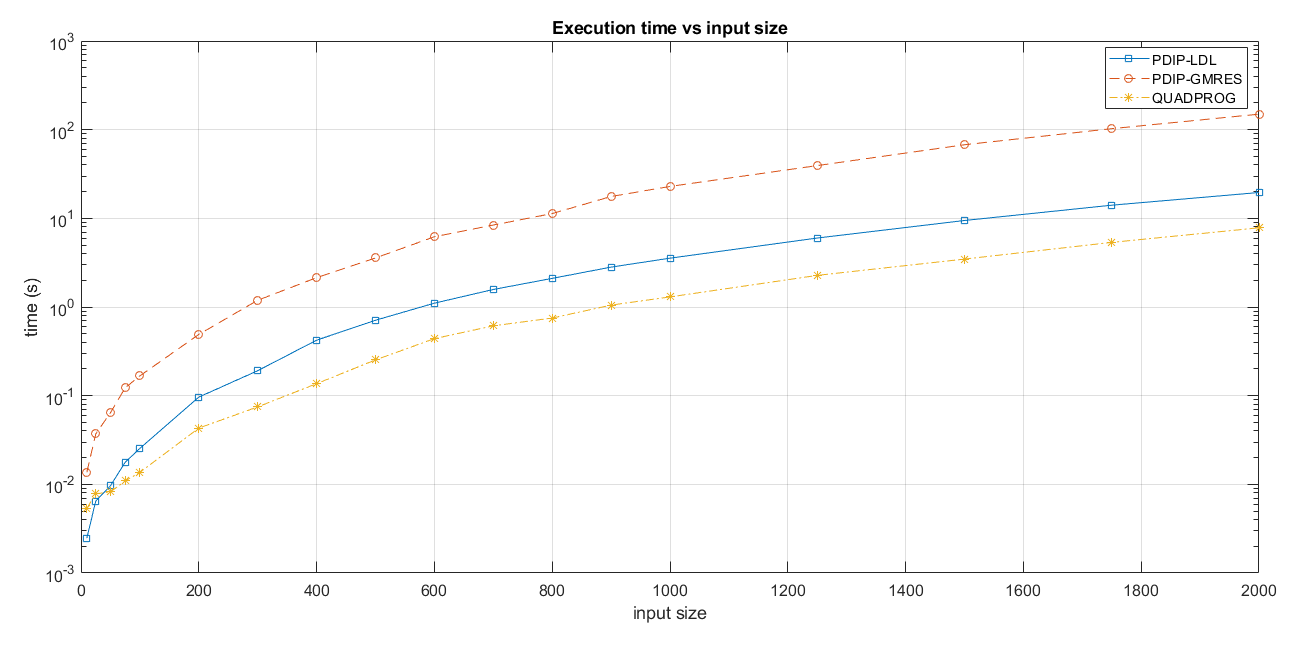
\includegraphics[height=4.3cm]{img/MU1.png}
    \caption{Confronto fra i tre metodi con asse delle y in \textit{log-scale}.\label{fig:exp111}}
    \end{subfigure}%
    ~ 
    \begin{subfigure}[h]{0.5\textwidth}
        \centering
               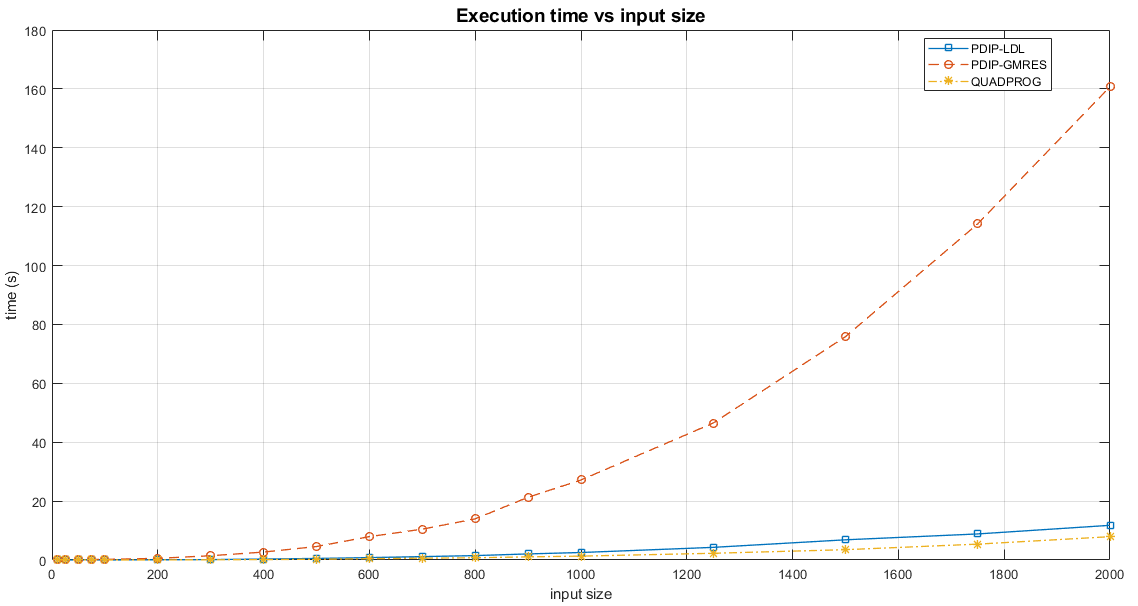
\includegraphics[height=4.3cm]{img/MU10.png}
    \caption{Confronto fra i tre metodi. \label{fig:exp112}}
    \end{subfigure}
    ~\newline
     \begin{subfigure}[h]{0.8\textwidth}
        \centering
                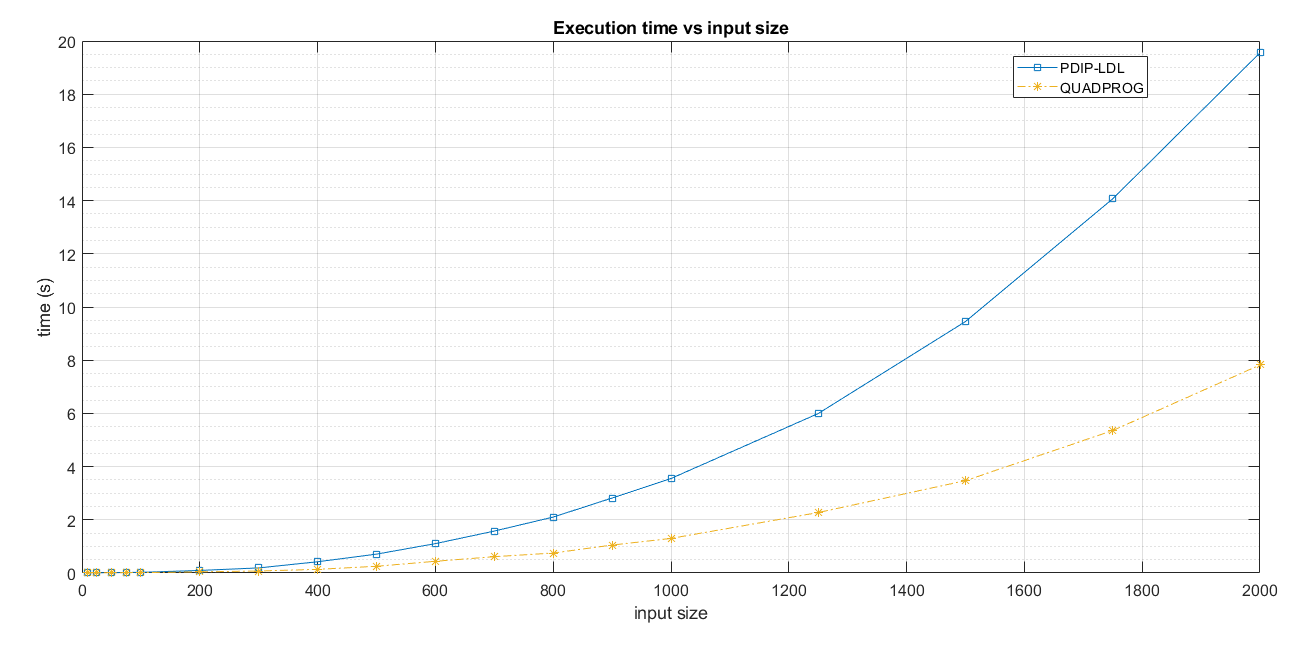
\includegraphics[height=7cm]{img/MU11.png}
    \caption{Grafico di confronto fra PIDP-LDL e QUADPROG. \label{fig:exp113}}
    \end{subfigure}
    \caption{Tempo di esecuzione, in secondi, all'aumentare della dimensione del problema $n$. \label{fig:exp1}}
\end{figure}



La Figura \ref{fig:exp1} ci permette di confrontare i tempi di completamento dei metodi analizzati; possiamo notare che l'andamento è esponenziale rispetto ad $n$ per tutti e tre i metodi.
In particolare:
\begin{itemize}
    \item in Fig.\ref{fig:exp112} la curva relativa al metodo PDIP-GMRES cresce con un esponente maggiore rispetto agli altri due metodi, questo a causa della presenza di metodo iterativo al suo interno, ossia GMRES, che all'aumentare di $n$ dovrà approssimare la soluzione di un sistema sempre più grande.
    
    \item confrontando i due metodi più veloci in Fig.\ref{fig:exp113} e Tab.\ref{tab:ldlqp2} possiamo notare come la nostra implementazione abbia scalabilità paragonabile a quella di QUADRPROG a meno di un fattore $\approx\times2.24$.

\end{itemize}

\begin{table}[!h]
\centering
\begin{tabular}{|l|c|c|c|c|c|c|c|c|}
\hline \textbf{input size}                  & \textbf{50}  & \textbf{75}  & \textbf{100} & \textbf{200}  & \textbf{300}  & \textbf{400}  & \textbf{500}  & \textbf{600}  \\\hline
\textbf{PDIP-LDL}                    & 0.0096       & 0.0177       & 0.0255       & 0.0964        & 0.1913        & 0.4224        & 0.7092        & 1.1048        \\
\textbf{QUADPROG}                    & 0.0082       & 0.0109       & 0.0136       & 0.0431        & 0.0747        & 0.1366        & 0.2531        & 0.4398        \\
\textbf{slowfactor} & \textbf{1.1734}       & 1.6271       & 1.8670       & 2.2362        & 2.559547        & \textbf{3.0921}        & 2.8019        & 2.5121        \\ \hline
\textbf{input size}                  & \textbf{700} & \textbf{800} & \textbf{900} & \textbf{1000} & \textbf{1250} & \textbf{1500} & \textbf{1750} & \textbf{2000} \\\hline
\textbf{PDIP-LDL}                    & 1.5736       & 2.1028       & 2.8189       & 3.5534        & 5.9961        & 9.4543        & 14.0684        & 19.5569       \\
\textbf{QUADPROG}                    & 0.6135       & 0.7508       & 1.0506       & 1.2995        & 2.2731        & 3.4718        & 5.3564        & 7.8202        \\
\textbf{\textit{slowfactor}} & 2.5694       & 2.8007       & 2.6831       & 2.7347        & 2.6378        & 2.7231        & 2.6265        & 2.5008  \\\hline     
\end{tabular}
    \caption{Tabelle contenenti la media dei tempi di esecuzione (s) di PDIP-LDL e QUADPROG relativi al primo sotto-esperimento. \label{tab:ldlqp2}}
    \end{table}
   
    
\begin{table}[!h]
\centering
\begin{tabular}{|l|c|c|c|c|c|c|c|c|}\hline
\textbf{input size} & \textbf{50}  & \textbf{75}  & \textbf{100} & \textbf{200}  & \textbf{300}  & \textbf{400}  & \textbf{500}  & \textbf{600}  \\\hline
\textbf{PDIP-LDL}   & 19.68\%      & 12.3\%      & 7.51\%      & 22.83\%        & 0.84\%        & 0.82\%        & 0.44\%        & 0.66\%        \\
\textbf{QUADPROG}   & 18.98\%      & 13.39\%      & 5.35\%      & 19.55\%        & 4.09\%        & 1.8\%        & 5.94\%       & 1.42\%        \\\hline
\textbf{input size} & \textbf{700} & \textbf{800} & \textbf{900} & \textbf{1000} & \textbf{1250} & \textbf{1500} & \textbf{1750} & \textbf{2000} \\\hline
\textbf{PDIP-LDL}   & 2.69\%       & 0.4\%       & 0.59\%       & 0.51\%        & 0.44\%        & 0.45\%        & 1\%        & 0.9\%        \\
\textbf{QUADPROG}   & 1.32\%       & 3.66\%       & 1.2\%       & 0.79\%        & 1.07\%        & 1.26\%        & 4.47\%        & 0.64\%     \\  \hline
\end{tabular}
    \caption{Tabella contenente la deviazione standard dei tempi di esecuzione di PDIP-LDL e QUADPROG relativi al primo sotto-esperimento. \label{tab:ldlqp1.1}}
\end{table}

La Tab. \ref{tab:ldlqp1.1} mostra come le prestazioni ottenute sono stabili anche in termini di deviazione standard; si nota un leggero aumento di quest'ultima sulle istanze piccole del problema in quanto i tempi in gioco sono davvero piccoli e una piccola variazione incide maggiormente sulla metrica.

L'incremento dell'input-size non sembra invece influire in maniera significativa sul  numero di iterazioni necessarie alla convergenza dei metodi.
Il grafico in Fig.\ref{fig:exp1.2} mostra infatti come, a prescindere dal valore di $n$, PDIP impieghi circa 20 iterazioni mentre QUADPROG circa 7.

\begin{figure}[!h]
    \centering
    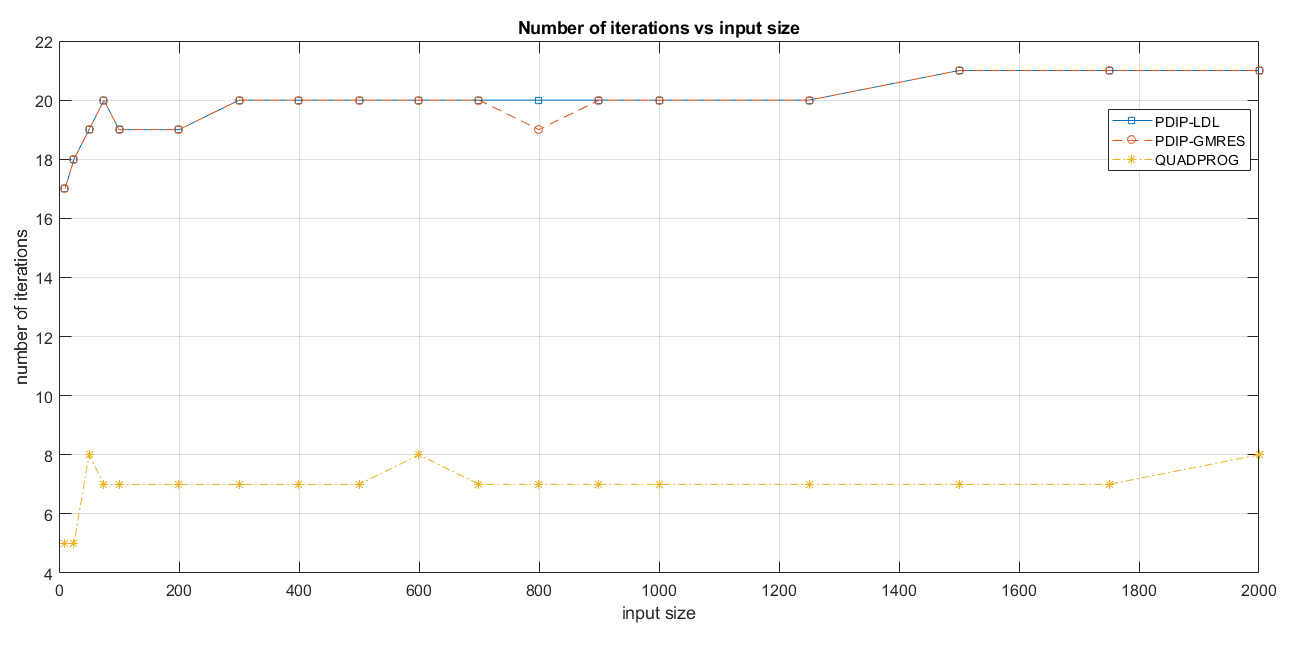
\includegraphics[width=\textwidth]{img/MU7.png}
    \caption{Il grafico mostra l'andamento del numero di iterazioni all'aumentare di $n$. \label{fig:exp1.2}}
\end{figure}

\subsection{Numero di Vincoli}

 In questo gruppo di esperimenti abbiamo voluto analizzare l'effetto che la variazione di $m$ ha sul tempo di convergenza dei metodi; $\delta$ ed $n$ rimangono fissati come in Tab. \ref{tab:param}.

\begin{figure}[h!]
    \centering
    \begin{subfigure}[h]{0.5\textwidth}
        \centering
        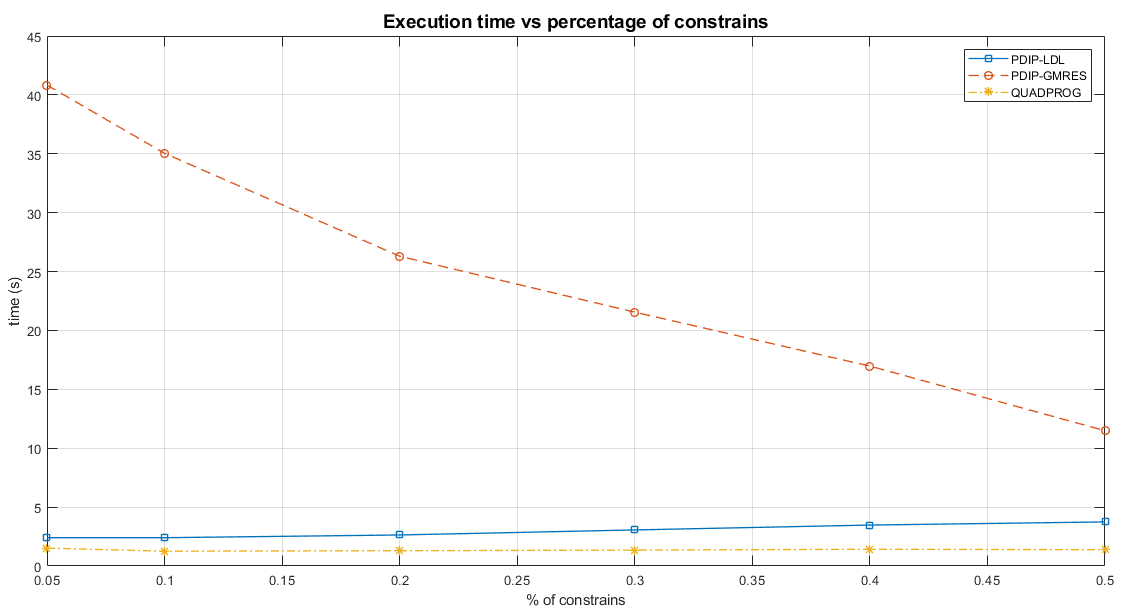
\includegraphics[width=\textwidth, height=2.42in]{img/MU2.png}
    \caption{Grafico di confronto fra i tempi di esecuzione dei tre metodi. \label{fig:exp2}}
    \end{subfigure}%
    ~ 
    \begin{subfigure}[h]{0.5\textwidth}
        \centering
         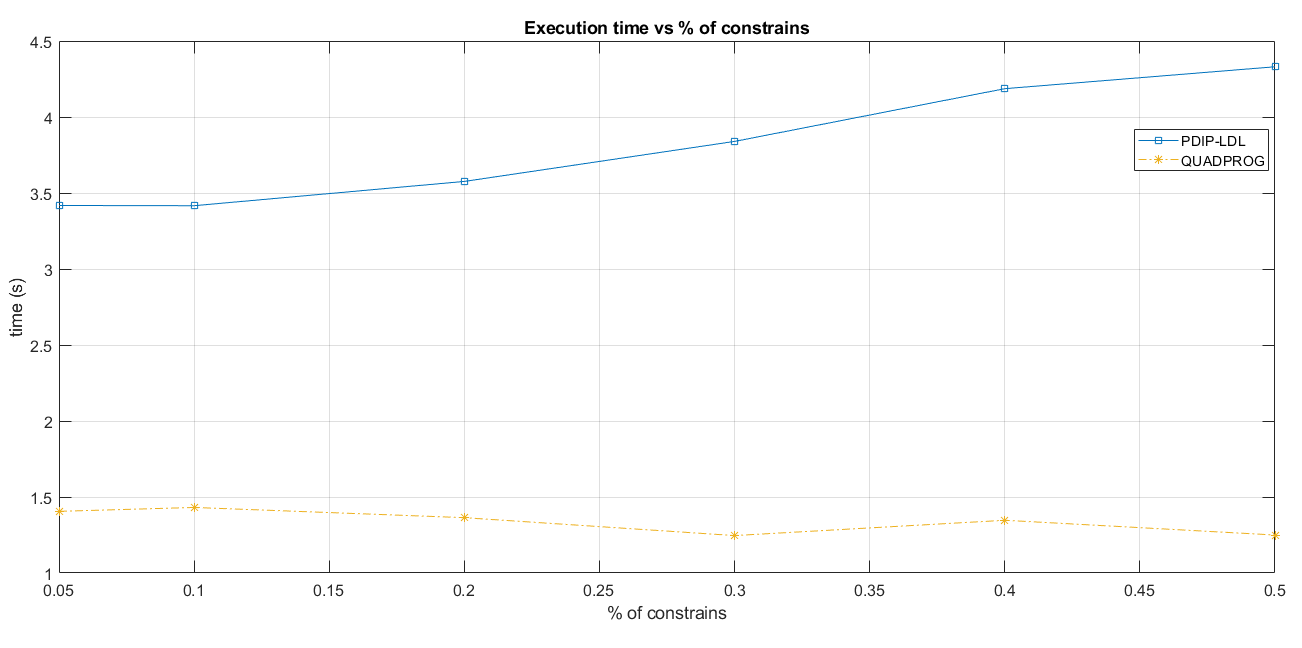
\includegraphics[width=\textwidth, height=2.4in]{img/MU3.png}
    \caption{Grafico di confronto fra PIDP-LDL e QUADPROG. \label{fig:exp2.1}}
    \end{subfigure}
    \caption{I grafici mostrano l'andamento del tempo di esecuzione, in secondi, all'aumentare del numero dei vincoli $m$; espresso in percentuale rispetto ad $n$. \label{fig:exp22}}
\end{figure}
 
In Fig.\ref{fig:exp2} i tempi di convergenza di PDIP-GMRES migliorano all'aumentare del numero di vincoli; questo perchè GMRES è più efficiente su matrici sparse e poichè il numero di elementi non-nulli in $A$ è sempre $n$, all'aumentare di $m$, la sparsità di $A$ aumenta, come di conseguenza quella del sistema KKT da risolvere.

Confrontando invece PDIP-LDL e QUADPROG in Fig.\ref{fig:exp2.1}, notiamo come l'aumentare del numero di vincoli impatti in modo negativo sulle performance della nostra implementazione, probabilmente a causa dell'aumento della dimensione del sistema da risolvere che penalizza l'approccio diretto. Il tempo di convergenza di QUADPROG invece rimane costante all'aumentare di $m$, di conseguenza lo slowfactor aumenta al variare di $m$, rimanendo però compreso nell'intervallo $[2.3, 3.5]$.

La Tabella \ref{tab:ldlqp2} conferma la stabilità del nostro metodo più veloce: si osservano infatti deviazioni standard trascurabili, dello stesso ordine di grandezza di QUADPROG.

\begin{table}[!h]
\centering
\begin{tabular}{c|c|c|c|c|c|c}

$\mathbf{m}$            & \textbf{0.05} & \textbf{0.1} & \textbf{0.2} & \textbf{0.3} & \textbf{0.4} & \textbf{0.5} \\ \hline
\textbf{PDIP-LDL}                    & $3.417 \pm 11.5\%$       & $3.416 \pm 11.5\%$       & $3.576     \pm 11\%$   & $3.839 \pm 10.2\%$      & $4.186 \pm 9.4\%$      & $4.33 \pm 9.1\%$       \\
\textbf{QUADPROG}                    & $1.405 \pm 5.2\%$       & $1.431 \pm 5.4\%$       & $1.364 \pm 5.7\%$       & $1.246 \pm 6.2\%$       & $1.346 \pm 5.7\%$       & $1.249 \pm 6.2\%$       \\
\textbf{\textit{slowfactor}} &2.431        & \textbf{2.387}      & 2.621       & 3.08       & 3.108       & \textbf{3.464} 
\end{tabular}
\caption{Tabella contenente media e deviazione standard dei tempi di esecuzione (s) di PDIP-LDL e QUADPROG relativi al secondo sotto-esperimento.\label{tab:ldlqp2}}
\end{table}

Infine, osserviamo che in Fig. \ref{fig:exp2.2} il numero di iterazioni diminuisce all'aumentare di $m$, questo però non vale per QUADPROG il cui numero di iterazioni non viene influenzato dalla frazione di vincoli rispetto alla dimensione dell'input.


\begin{figure}[!h]
    \centering
    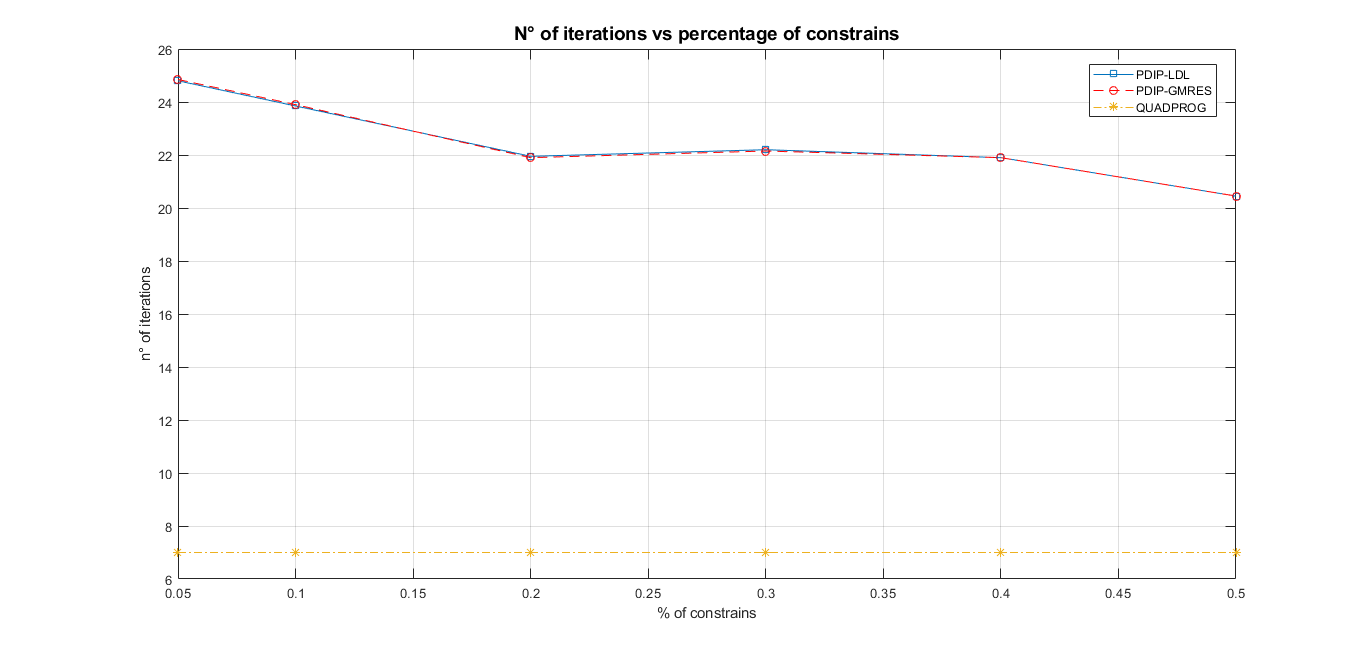
\includegraphics[width=\textwidth]{img/MU8.png}
    \caption{Numero di iterazioni all'aumentare di $m$. \label{fig:exp2.2}}
\end{figure}


\subsection{Densità}

 In questo gruppo di esperimenti abbiamo voluto testare qualora la densità della matrice $Q$ avesse effetti sui tempi di convergenza e il numero di iterazioni dei vari approcci coinvolti nella nostra analisi.

\begin{figure}[!h]
    \centering
    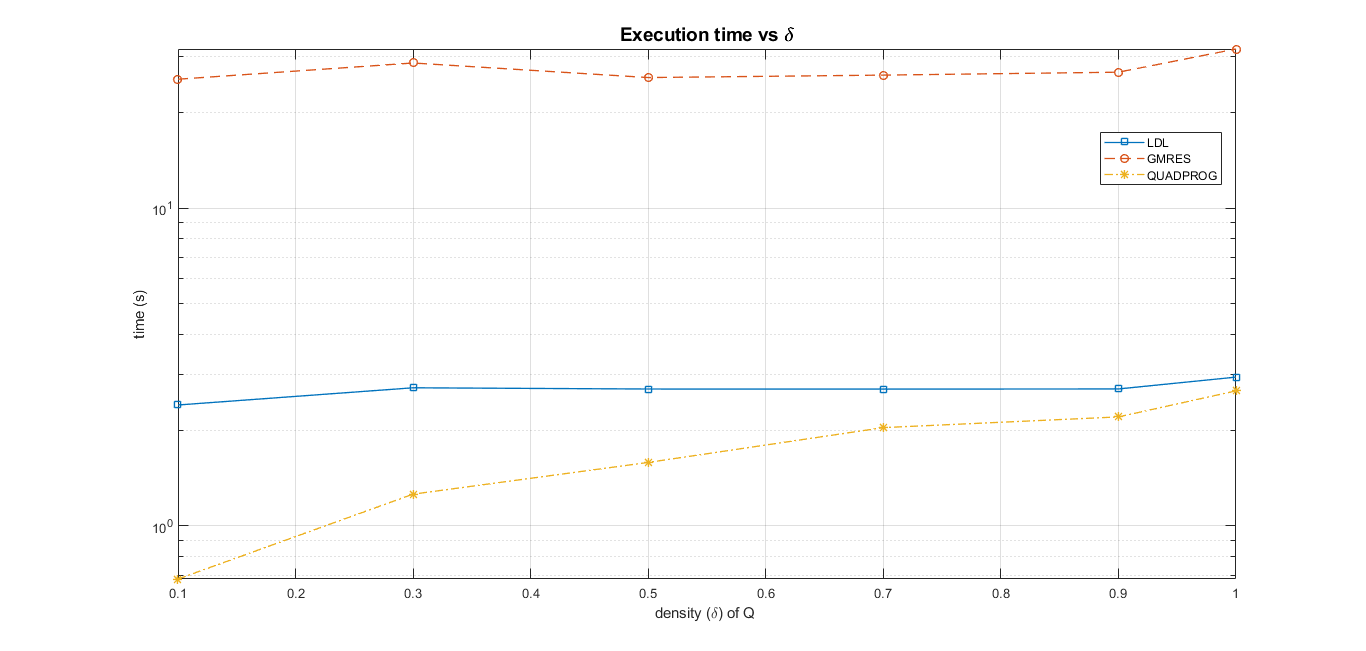
\includegraphics[width=0.9\textwidth, height=7.3cm]{img/MU4.png}
    \caption{Tempo di esecuzione dei tre metodi all'aumentare della densità ($\delta$) di $Q$. \label{fig:exp3.1}}
\end{figure}
 
Da Fig.\ref{fig:exp3.1} si evince che l'aumento di $\delta$ ha un impatto critico sulle prestazioni di PDIP-GMRES, mentre incide in maniera minore su quelle di PIDP-LDL e QUADPROG. Questo è ancora una volta conseguenza dell'utilizzo di GMRES che predilige matrici più sparse possibili. 

 Confrontando pù in dettaglio i tempi di PDIP-LDL e QUADPROG in Tab. \ref{tab:ldlqp3}:
 \begin{itemize}
     \item il tempo di completamento della versione con risoluzione diretta della nostra implementazione inizialmente aumenta, poi diminuisce per poi stabilizzarsi introno a valori simili a quelli di QUADPROG
     \item il tempo di completamento di QUADPROG, invece, aumenta monotonamente
     \item di conseguenza lo slowfactor è massimo in corrispondenza del valore minimo di $\delta$, minimo viceversa; in generale la nostra implementazione è più lenta di un fattore $\approx \times2.1$.
 \end{itemize}
\begin{table}[!h]
\centering
\begin{tabular}{l|c|c|c|c|c|c}
\textbf{density}                     & \textbf{0.1} & \textbf{0.3} & \textbf{0.5} & \textbf{0.7} & \textbf{0.9} & \textbf{1.0} \\ \hline
\textbf{PDIP-LDL}                    & $1.882 \pm 0.5\%$       & $3.026 \pm 1.5\%$       & $4.24  \pm 0.3\%$       & $4.943 \pm 0.3\%$       & $2.626 \pm 5.9\%$       & $2.489  \pm 1.6\%$       \\
\textbf{QUADPROG}                    & $0.634  \pm 1.5\%$      & $1.33  \pm 1.2\%$       & $1.527 \pm 0.7\%$       & $1.942 \pm 1\%$       & $2.377 \pm 1.1\%$       & $2.441 \pm 0.9\%$       \\
\textbf{\textit{slowfactor}} & \textbf{2.966}       & 2.274       & 2.775       & 2.522       & 1.104       & \textbf{1.009}
\end{tabular}
\caption{Tabella contenente media e deviazione standard dei tempi di esecuzione (s) di PDIP-LDL e QUADPROG relativi al terzo sotto-esperimento. \label{tab:ldlqp3}}
\end{table}

 Infine in Fig.\ref{fig:exp3.2} il numero di iterazioni necessarie convergenza rimane stabile rispetto alla variazione di densità di $Q$ in tutti i metodi testati, con valori identici a quelli osservati nella recedente sezione. 
 

\begin{figure}[!h]
    \centering
    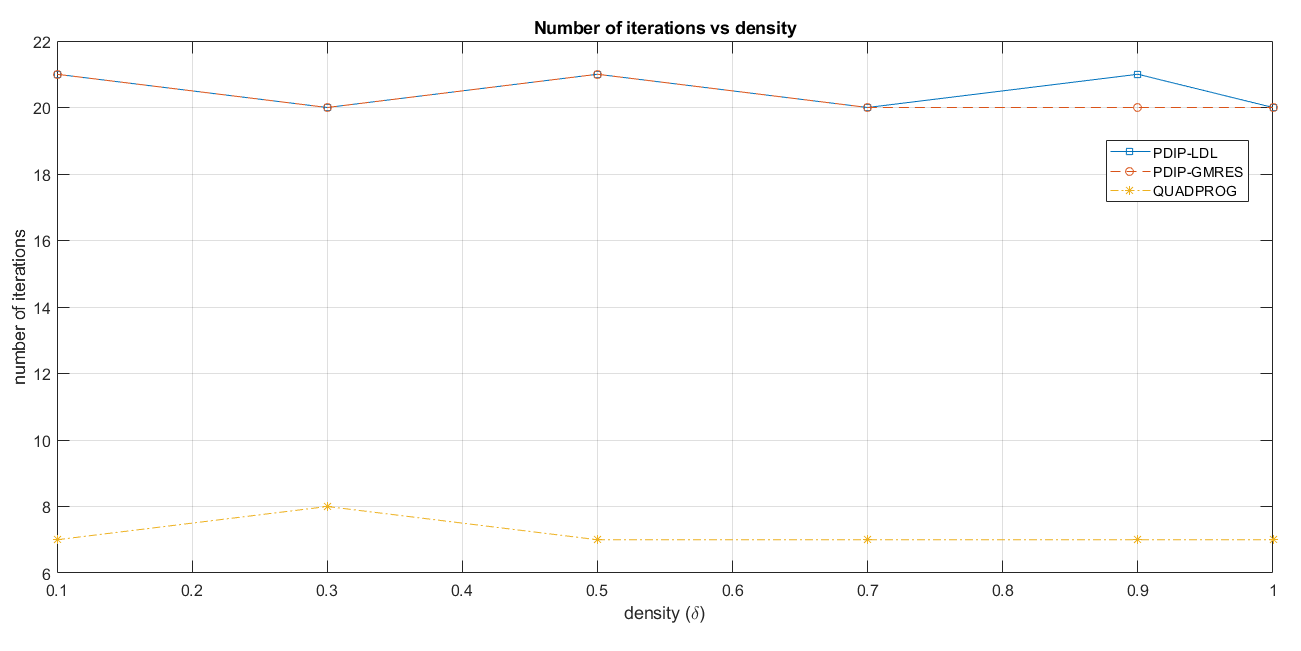
\includegraphics[width=0.9\textwidth, height = 6.5cm]{img/MU9.png}
    \caption{Grafico dell'andamento del numero di iterazioni all'aumentare di $\delta$. \label{fig:exp3.2}}
\end{figure}

\subsection{Convergenza e Accuratezza della Soluzione}

Per i risultati in questa sezione sono state effettuate 20 esecuzioni fissando il problema come in Tab. \ref{tab:param}.
Per analizzare la convergenza dell'implementazione proposta, abbiamo collezionato i complementary gap ad ogni iterazione di PDIP sia in versione GMRES, che LDL.

Il grafico in Fig. \ref{fig:gap} mostra come varia - in scala logaritmica sull'asse delle y - ad ogni iterazione la media dei complementary gap: in entrambe le varianti della nostra implementazione il gap decresce monotonamente ad ogni iterazione successiva alla seconda e le prestazioni sono in linea con quelle attese.

\begin{figure}[!h]
    \centering
    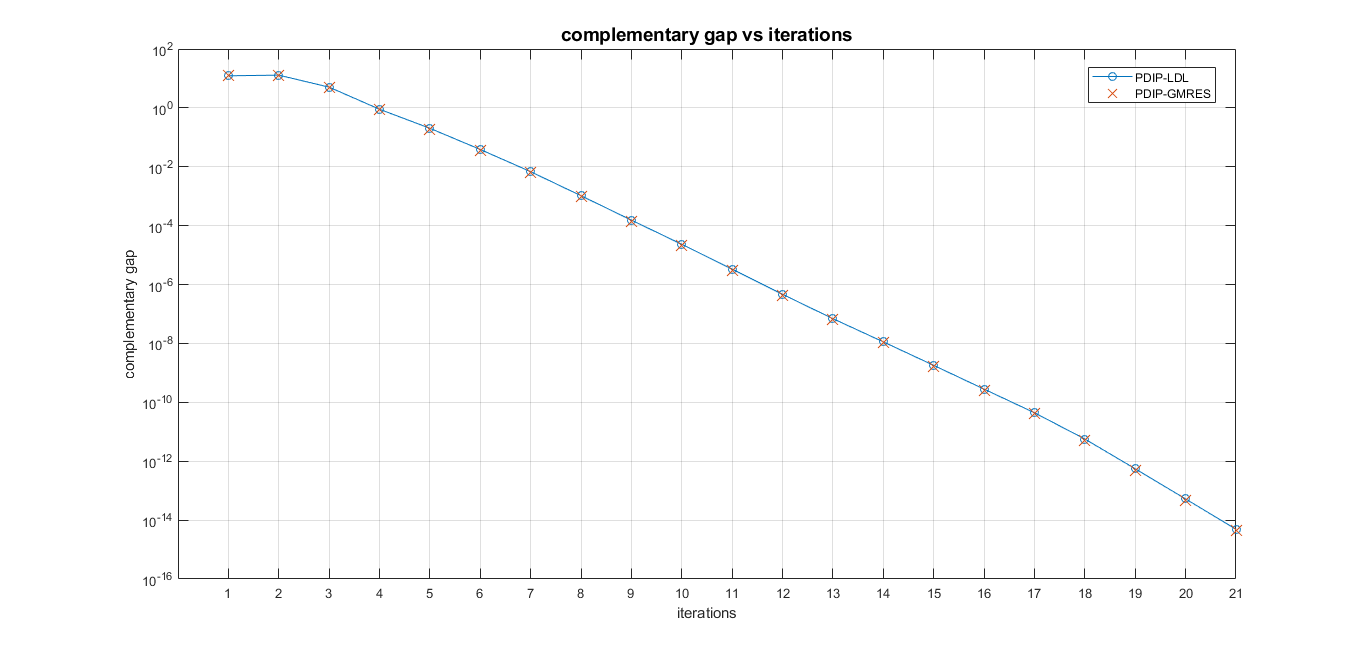
\includegraphics[width=\textwidth, height = 8cm]{img/MU6.png}
    \caption{Andamento del gap (in \textit{log-scale} sull'asse delle y) all'aumentare delle iterazioni. \label{fig:gap}}
\end{figure}

La seconda parte di questo esperimento ha l'obiettivo di valutare l'accuratezza della soluzione $(x, \lambda_{eq}, \lambda_s)$ dal nostro metodo. A questo proposito confrontiamo i residui finali e le triple restituite da PDIP-GMRES e PDIP-LDL fra di loro e con quella di QUADPROG. 

Come metrica di confronto per le triple abbiamo scelto di usare la norma della differenza fra i vettori soluzione $\norm{\delta_v}$ :

\begin{equation}\label{ep:acc}
     \norm{v_{M1} - v_{M2}} \;\;\;\;\;\;\;\;\; \mathrm{con} \;\;\; v\in \{ x, \lambda_{eq}, \lambda_s\} \;\; \mathrm{e} \;\; M_i \in \{{\scriptsize\mathit{PDIP-LDL},\; \mathit{PDIP-GMRES}, \; \mathit{QUADPROG}}\}
\end{equation}

In Tab. \ref{tab:normx} e \ref{tab:norml} sono riportate medie e deviazioni standard - su 20 esecuzioni - delle metriche, calcolate come in \ref{ep:acc}, rispettivamente per i vettori $x$ e $\lambda$.   

\begin{table}[!h]
\centering
\begin{tabular}{c|c|l|c}
$\mathbf{\norm{\delta x}}$ & \multicolumn{2}{c|}{\textbf{PDIP-GMRES}}         & \textbf{QUADPROG}          \\ \hline
\textbf{PDIP-LDL}            & \multicolumn{2}{c|}{$4.2927\cdot10^{-13}\pm0\%$} & $5.4785\cdot10^{-3}\pm0\%$ \\ \hline
\textbf{PDIP-GMRES}          & \multicolumn{2}{c|}{}                            & $5.4785\cdot10^{-3}\pm0\%$
\end{tabular}
\caption{Media e deviazione standard, sulle 20 ripetizioni, della norma della differenza fra i vettori soluzione.\label{tab:normx}}
\end{table}

\begin{table}[!h]
\begin{tabular}{c|c|c|c|c|}
      $\mathbf{\norm{\delta\lambda}}$             & \multicolumn{2}{c|}{\textbf{PDIP-LDL}}                                        & \multicolumn{2}{c|}{\textbf{PDIP-GMRES}}                                      \\ \hline
\textbf{PDIP-GMRES} & $1.6224\cdot10^{-13}\pm0\%$          & $7.4955\cdot10^{-13}\pm0\%$         & \multicolumn{2}{c|}{ }                                                        \\ 
\textbf{QUADPROG}   & $2.1561\cdot10^{-3}\pm0\%$            & $7.0229\cdot10^{-3}\pm0\%$            & $2.1561\cdot10^{-3}\pm0\%$            & $7.0229\cdot10^{{-3}}\pm0\%$          \\
                    & $\norm{ \delta\lambda_{eqlin} }$ & $\norm{ \delta\lambda_{s} }$ & $\norm{ \delta\lambda_{eqlin} }$ & $\norm{ \delta\lambda_{s} }$
\end{tabular}
\caption{Media e deviazione standard, sulle 20 ripetizioni, della norma della differenza fra i moltiplicatori lagrangiani soluzione dei metodi testati.\label{tab:norml}}
\end{table}

\begin{table}[!h]
\centering
\begin{tabular}{c|c|c}
\textbf{}           & $\mathbf{\norm{r_p}}$ & $\mathbf{\norm{r_d}}$ \\\hline
\textbf{PDIP-LDL} &      $1.2462\cdot10^{-15} \pm0\%$                 &           $3.1114\cdot10^{-14} \pm0\%$             \\\hline
\textbf{PDIP-GMRES}   &        $1.0181\cdot10^{-13} \pm0\%$               &            $7.2054\cdot10^{-13} \pm0\%$           \\\hline
\textbf{QUADPROG}   &      $1.3323\cdot10^{-15} \pm0\%$                &            $1.0767\cdot10^{-14} \pm0\%$   \\    
\end{tabular}
\caption{Tabella che riporta la media e deviazione standard su 20 esecuzioni della norma dei residui primali e duali finali dei tre metodi in analisi.}
\label{tab:res}
\end{table}

Le soluzioni ottenute dall'esecuzione diretta e iterativa di PDIP risultano pressocchè identiche: sia $\norm{\delta x}$ che $\norm{\delta\lambda}$ sono dell'ordine di $10^{-13}$; ed entrambe queste soluzioni sono uguali a quella trovata da QUADPROG a meno di un fattore di $10^{-3}$.

La Tabella \ref{tab:res} conferma ulteriormente la precisione della nostra implementazione: 
\begin{itemize}
    \item l'accuratezza raggiunta è paragonabile a quella di QUADPROG, osserviamo infatti che PDIP-LDL risolve il problema con residuo primale e duale dello stesso ordine di grandezza di QUADPROG, PDIP-GMRES invece è meno accurato di circa un ordine di grandezza su entrambi i residui;
    
    probabilmente potrebbe raggiungere precisione dello stesso ordine di grandezza di QUADPROG scegliendo una soglia $\eps$ più bassa rispetto a quella usata nei nostri esperimenti ($10^{-14}$), impiegando però più iterazioni e risultando più lento
    \item la deviazione standard è nulla in ogni tabella in questa sezione, quindi la nostra implementazione, fissato un problema, restituisce sempre la stessa soluzione, come anche QUADPROG; tuttavia durante il resto della fase sperimentale abbiamo osservato deviazioni standard (sui tempi di convergenza) più alte per la nostra implementazione. Questo fenomeno può essere spiegato dalla presenza di una parte randomica nel nostro metodo, precisamente in \ref{eq:startl} durante la generazione della tripla iniziale: $\lambda_{eq}$ viene inizializzato con reali casuali, influenzando anche l'inizializzazione di $\lambda_s$; QUADPROG invece inizializza sempre $(x^0, \lambda_{eq}^0, \lambda_s^0) = 1$, con risultati finali, in termini di tempo di convergenza, di conseguenza più simili fra loro.
\end{itemize}

Concludendo la nostra implementazione, sia in versione diretta, che iterativa, può essere considerata stabile e accurata rispetto alla built-in di \texttt{MATLAB} sia in termini di tempi ed iterazioni di convergenza, che di precisione del risultato finale.
\section{Conclusioni}
riassunto results:
\begin{itemize}
    \item la nostra implementazione ha prestazioni, in termini di tempo di esecuzione e numero di iterazioni, che si avvicinano di molto a quelle dell'implementazione built-in di \texttt{MATLAB}
    \item  in partiolare PDIP-GMRES risulta il più lento, principalmente perchè contiene la risoluzione iterativa dell'\textit{augmented KKT}. 
    
    Tuttavia le prestazioni di questo metodo migliorano significamene all'aumentare del numero di vincoli, e quindi di righe, in $A$; questo accade perché la struttura della matrice nel nostro problema induce una diminuzione della densità della matrice stessa, all'aumentare di $m$. E GMRES funziona meglio su matrici sparse.
    
    \item LDL ha prestazioni sempre paragonabili a QUADPROG: è più lento in media di un fattore $\approx\times2$, soffre più di QUADPROG l'aumento del numero di vincoli, ma è molto più stabile all'aumentare della densità della matrice $Q$.
    
    \item QUADPROG fa circa la metà delle iterazioni rispetto alle nostre implementazioni, a prescindere dai parametri.ì

\end{itemize}
\newpage
\bibliographystyle{plain}
\bibliography{references}
\end{document}
